%%%%%%%%%%%%%%%%%%%%%%%%%%%%%%%%%%%%%%%%%
% baposter Landscape Poster
% LaTeX Template
% Version 1.0 (11/06/13)
%
% baposter Class Created by:
% Brian Amberg (baposter@brian-amberg.de)
%
% This template has been downloaded from:
% http://www.LaTeXTemplates.com
%
% License:
% CC BY-NC-SA 3.0 (http://creativecommons.org/licenses/by-nc-sa/3.0/)
%
%%%%%%%%%%%%%%%%%%%%%%%%%%%%%%%%%%%%%%%%%

%----------------------------------------------------------------------------------------
%	PACKAGES AND OTHER DOCUMENT CONFIGURATIONS
%----------------------------------------------------------------------------------------

\documentclass[landscape,a0paper,fontscale=0.22]{baposter} % Adjust the font scale/size here

\usepackage{graphicx} % Required for including images
\graphicspath{{figures/}} % Directory in which figures are stored

\usepackage{amsmath} % For typesetting math
\usepackage{amssymb} % Adds new symbols to be used in math mode

\usepackage{booktabs} % Top and bottom rules for tables
\usepackage{enumitem} % Used to reduce itemize/enumerate spacing
\usepackage{palatino} % Use the Palatino font
\usepackage[font=small,labelfont=bf]{caption} % Required for specifying captions to tables and figures

\usepackage{multicol} % Required for multiple columns
\setlength{\columnsep}{1.5em} % Slightly increase the space between columns
\setlength{\columnseprule}{0mm} % No horizontal rule between columns

\usepackage{tikz} % Required for flow chart
\usetikzlibrary{shapes,arrows} % Tikz libraries required for the flow chart in the template

\newcommand{\compresslist}{ % Define a command to reduce spacing within itemize/enumerate environments, this is used right after \begin{itemize} or \begin{enumerate}
\setlength{\itemsep}{1pt}
\setlength{\parskip}{0pt}
\setlength{\parsep}{0pt}
}

\definecolor{lightblue}{rgb}{0.145,0.6666,1} % Defines the color used for content box headers

\begin{document}

\begin{poster}
{
headerborder=closed, % Adds a border around the header of content boxes
colspacing=1em, % Column spacing
bgColorOne=white, % Background color for the gradient on the left side of the poster
bgColorTwo=white, % Background color for the gradient on the right side of the poster
borderColor=lightblue, % Border color
headerColorOne=black, % Background color for the header in the content boxes (left side)
headerColorTwo=lightblue, % Background color for the header in the content boxes (right side)
headerFontColor=white, % Text color for the header text in the content boxes
boxColorOne=white, % Background color of the content boxes
textborder=roundedleft, % Format of the border around content boxes, can be: none, bars, coils, triangles, rectangle, rounded, roundedsmall, roundedright or faded
eyecatcher=true, % Set to false for ignoring the left logo in the title and move the title left
headerheight=0.1\textheight, % Height of the header
headershape=roundedright, % Specify the rounded corner in the content box headers, can be: rectangle, small-rounded, roundedright, roundedleft or rounded
headerfont=\Large\bf\textsc, % Large, bold and sans serif font in the headers of content boxes
%textfont={\setlength{\parindent}{1.5em}}, % Uncomment for paragraph indentation
linewidth=2pt % Width of the border lines around content boxes
}
%----------------------------------------------------------------------------------------
%	TITLE SECTION 
%----------------------------------------------------------------------------------------
%
{
\includegraphics[height=6em]{julogo}} % First university/lab logo on the left
{\bf\textsc{EvoloPy: An Open-Source Nature-Inspired Optimization Framework in Python}\vspace{0.5em}} % Poster title
{\textsc{\{ H. Faris, I. Aljarah S. Mirjalili, P. A. Castillo and JJ Merelo \} \hspace{12pt}  U. of Granada}} % Author names and institution
{
\includegraphics[height=6em]{granadalogo}} % Second university/lab logo on the right

%----------------------------------------------------------------------------------------
%	OBJECTIVES
%----------------------------------------------------------------------------------------

\headerbox{Highlights}{name=objectives,column=0,row=0}{


\Large

\begin{enumerate}\compresslist
\item {\tt EvoloPy} is open source and cross-platform. 
\item Makes easier using metaheuristic algorithms for their own problems.
\item Or creating new ones.
\item Free software \url{https://github.com/7ossam81/EvoloPy}
\end{enumerate}

\vspace{0.3em} % When there are two boxes, some whitespace may need to be added if the one on the right has more content
}

%----------------------------------------------------------------------------------------
%	INTRODUCTION
%----------------------------------------------------------------------------------------





\headerbox{Framework Overview}{name=introduction,column=1,row=0
}{




EvoloPy provides a set of classical and recent nature-inspired metaheuristic optimizers with an easy-to-use interface. 

Main components of the framework are: 

\begin{itemize}\compresslist
\item The Optimizer: the main interface of the framework where users can select a list of optimizers to run in their experiment. The user can configure common parameters like population size and maximum iterations. 


\item The metaheuristic algorithms: this part includes the list of implemented optimizers. So far, the following eight algorithms have been implemented: 

\begin{itemize}\compresslist
\item  Particle Swarm Optimization (PSO), 
\item  Firefly Algorithm (FFA), 
\item  Gray Wolf Optimizer (GWO)
\item  Whale Optimization Algorithm (WOA)
\item  Multi-Verse Optimizer (MVO)
\item  Moth Flame Optimizer (MFO)
\item  Bat Algorithm (BAT)
\item Cuckoo Search Algorithm (CS) .
\end{itemize}



\item Benchmark functions and problem definitions: a set of benchmark problems commonly used for comparing metaheuristic algorithms. A user-defined cost function could be added to this list.

\item Results management: this component is responsible for exporting the results.

\end{itemize}}



%----------------------------------------------------------------------------------------
%	RESULTS 1
%----------------------------------------------------------------------------------------

\headerbox{Comparison with Matlab}{name=results,column=2,span=2,row=0,bottomaligned=introduction}{

\LARGE
NumPy rocks.
%------------------------------------------------

\begin{multicols}{2}
\vspace{1em}

\begin{center}
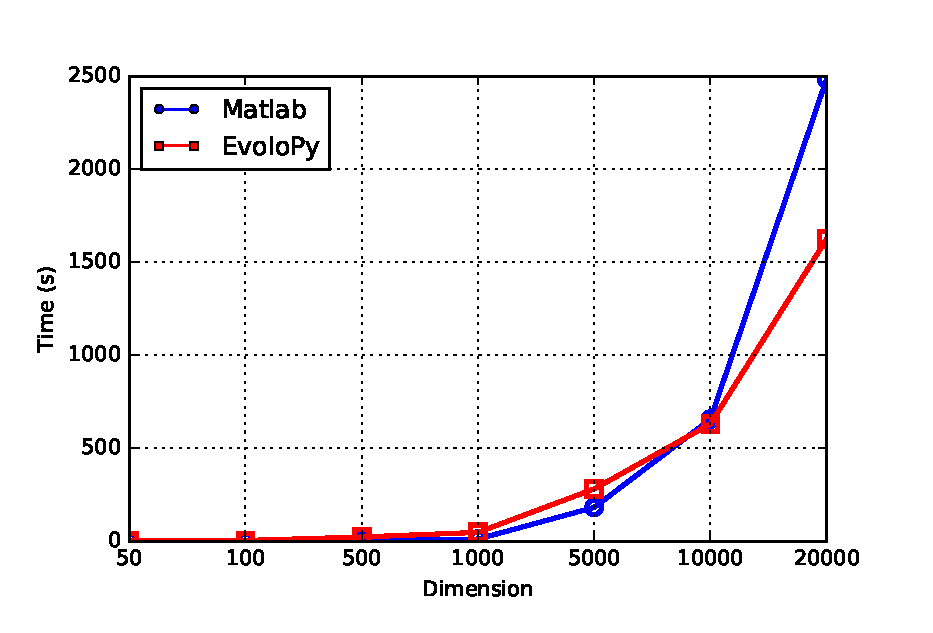
\includegraphics[width=0.95\linewidth]{PSO}
\captionof{figure}{PSO}
\label{fig:pso}
\end{center}


\begin{center}
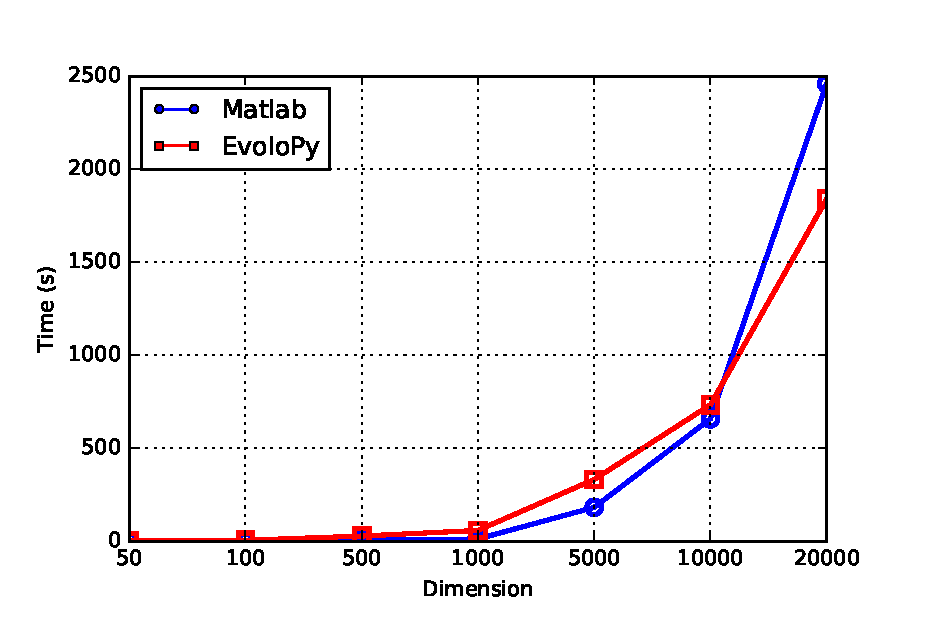
\includegraphics[width=0.95\linewidth]{GWO}
\captionof{figure}{GWO}
\label{fig:gwo}
\end{center}





\end{multicols}
}

%----------------------------------------------------------------------------------------
%	REFERENCES
%----------------------------------------------------------------------------------------

\headerbox{Contact}{name=references,column=0,above=bottom}{

KASIT, The University of Jordan
\{hossam.faris, i.aljarah\}@ju.edu.jo

ETSIIT-CITIC, University of Granada, Granada, Spain
\{pedro, jmerelo\}@geneura.urg.es

}

%----------------------------------------------------------------------------------------



\headerbox{Design issues}{name=conclusion,column=1,span=3,row=0,below=results}{

\begin{multicols}{2}

\begin{itemize}\compresslist

\item Populations are implemented as 2-dimensional arrays while individuals are implemented as 1-dimensional arrays. In EvoloPy, \texttt{Numpy} is chosen to define the populations and individuals in the optimizers. \texttt{Numpy} is an open-source extension to Python that provides common scientific computing and mathematical routines as pre-compiled and fast functions. \texttt{Numpy} has many things in common with Matlab. This makes it easier for researchers who are familiar with Matlab to use EvoloPy. 

\item  The core data structure \texttt{ndarray} from \texttt{Numpy} is used to define individuals and populations. For example, to define a randomly generated initial population with 50 individuals and 100 dimensions the following python line of code can be used

\texttt{initialPop = np.random.rand(50,100)}


\item With \texttt{Numpy} it is possible to perform vector operations in simple and compact syntax. For example, one of the common operations used in many metaheuristic algorithms is to check the boundaries of the elements of the individuals after updating them. This can be performed all at once with \texttt{Numpy} as follows:

\texttt{newPop=numpy.clip(oldPop, lb, ub)}

Where \texttt{lb} and \texttt{ub} are the upper and lower bounds respectively.




%\begin{figure*}
%\centerline{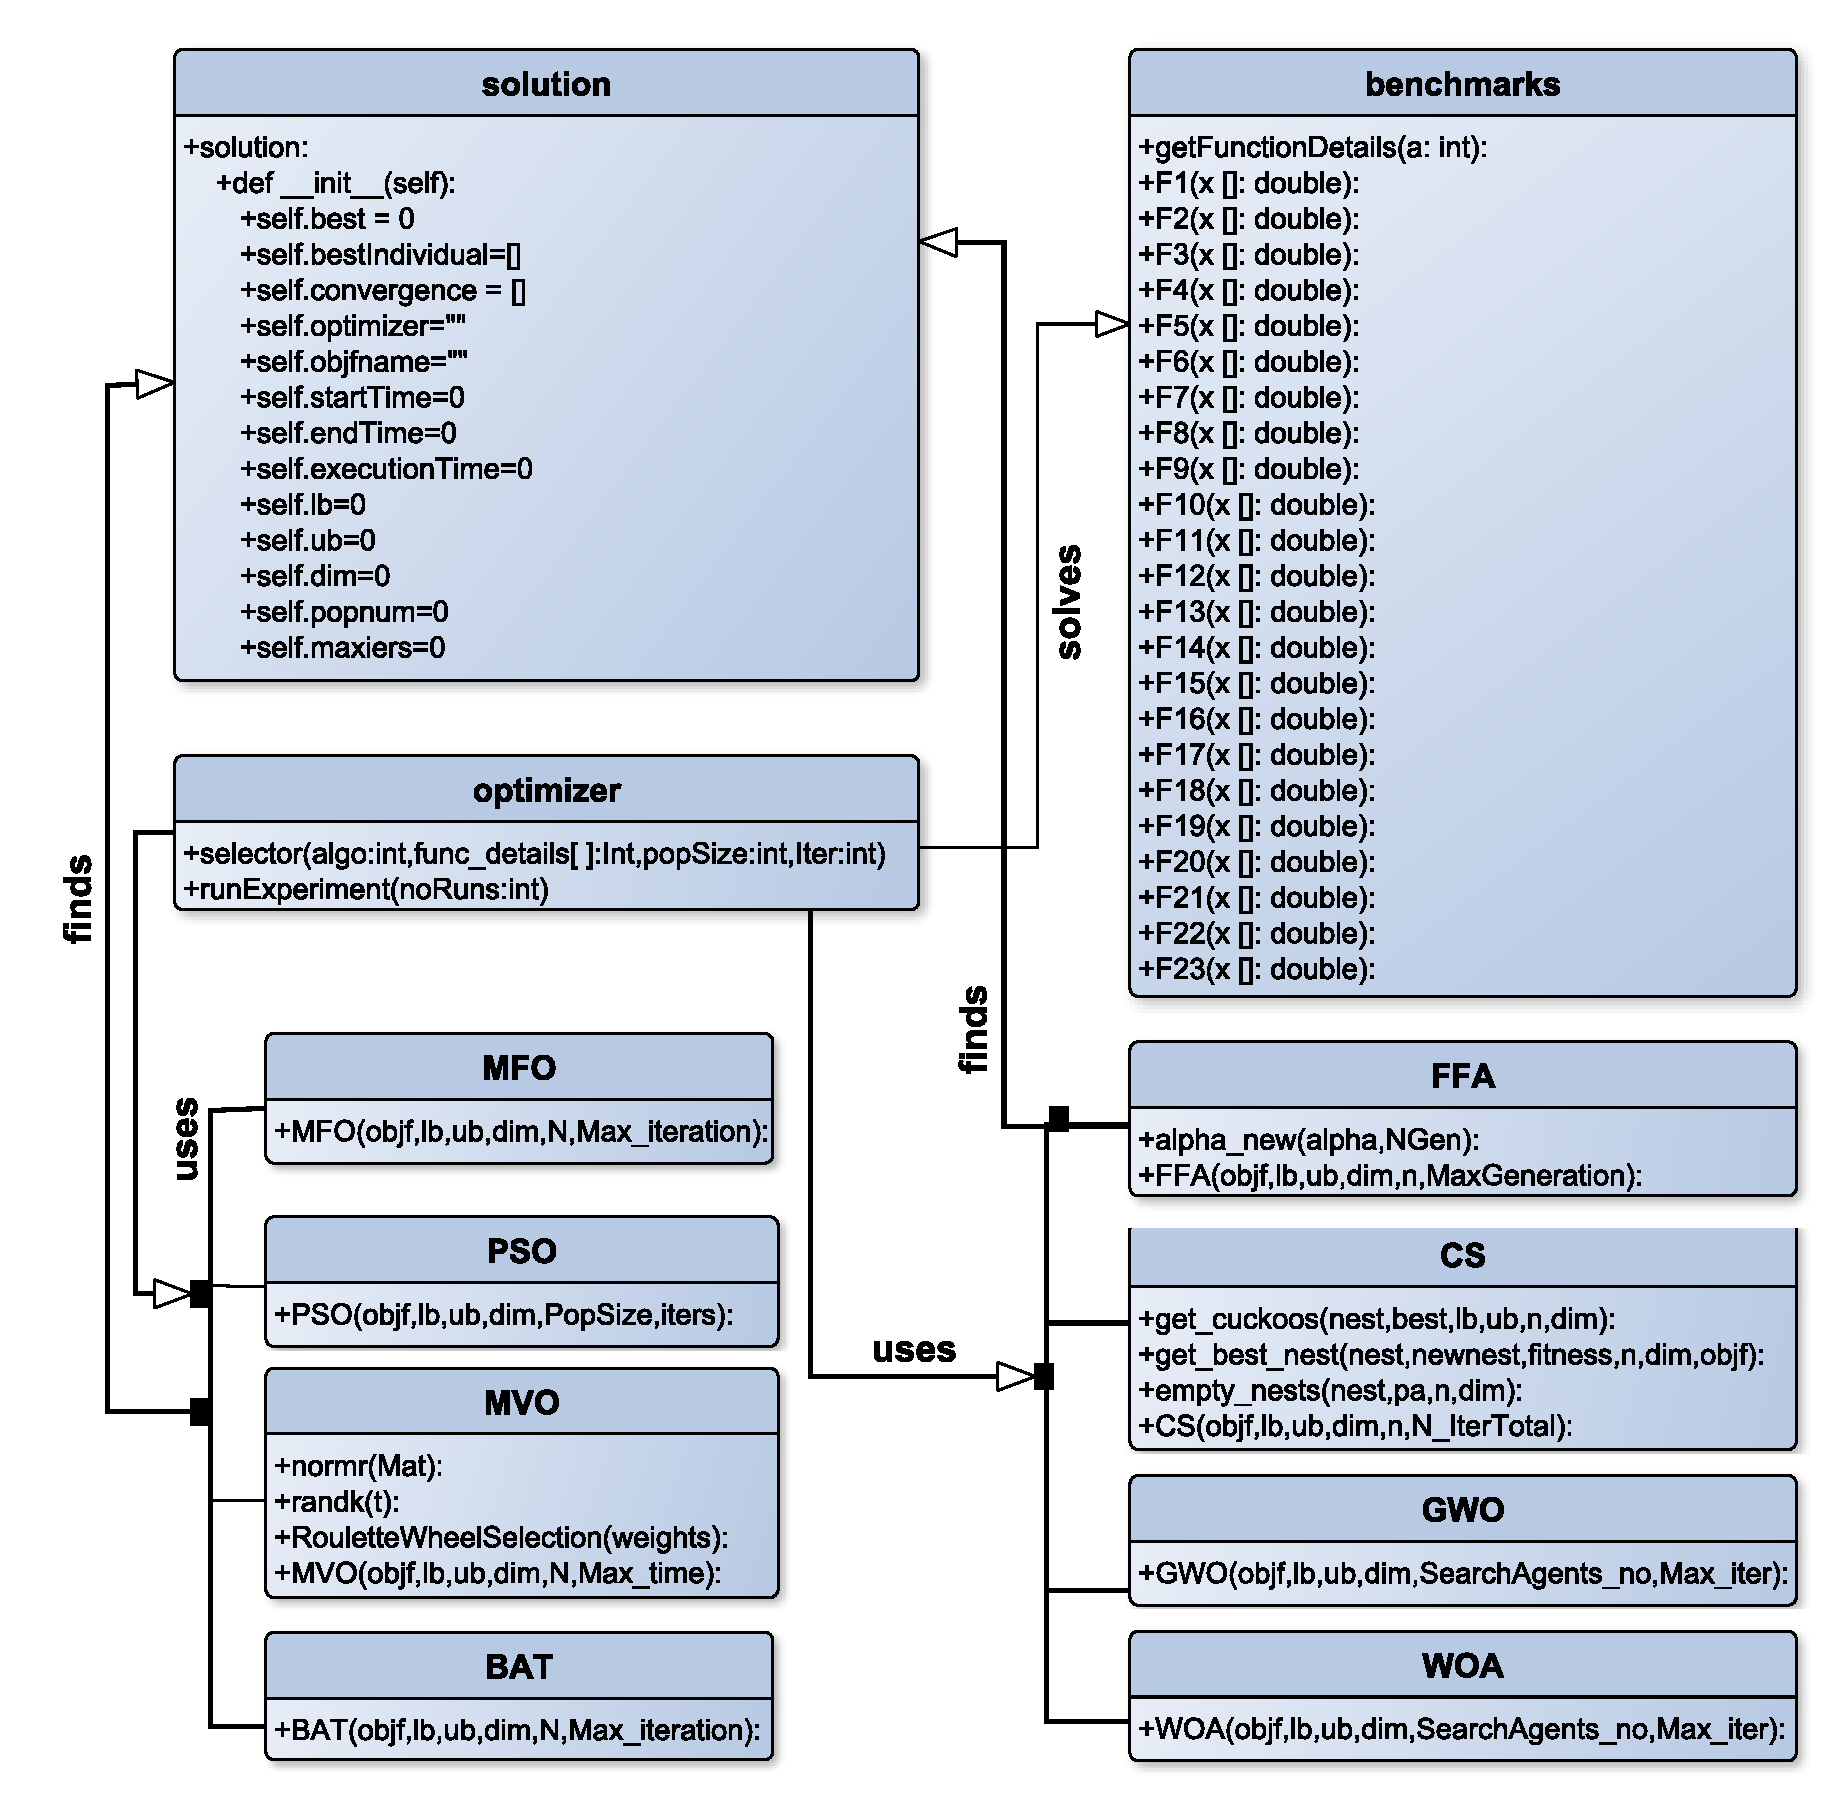
\includegraphics[scale=0.35]{classD}}
%\caption{Class diagram of the EvoloPy framework}
%\label{fig:framework}
%\end{figure*}

%To demonstrate the main components of EvoloPy framework we use the UML representation. A class diagram illustrating the EvoloPy components and their relationships is presented in Figure \ref{fig:framework}. 

\item  EvoloPy framework consists of eleven classes, three of them for coordinating and simplifying the optimization process, namely; optimizer, benchmarks, and solution. The other eight classes represent the optimizers.  

\end{itemize}

%------------------------------------------------

%\begin{itemize}\compresslist
%\item Pellentesque eget orci eros. Fusce ultricies, tellus et pellentesque fringilla, ante massa luctus libero, quis tristique purus urna nec nibh. Phasellus fermentum rutrum elementum. Nam quis justo lectus.
%\item Vestibulum sem ante, hendrerit a gravida ac, blandit quis magna.
%\item Donec sem metus, facilisis at condimentum eget, vehicula ut massa. Morbi consequat, diam sed convallis tincidunt, arcu nunc.
%\item Nunc at convallis urna. isus ante. Pellentesque condimentum dui. Etiam sagittis purus non tellus tempor volutpat. Donec et dui non massa tristique adipiscing.
%\end{itemize}

\end{multicols}
}


\headerbox{Why Python?}{name=method,column=0,below=objectives}{ % This block's bottom aligns with the bottom of the conclusion block

\begin{itemize}\compresslist
\item  Python is a general purpose scripting language which has a clear and simple syntax. 

\item  With the rapid development of open source scientific computing libraries and packages, Python became as one of the most popular and powerful languages for scientific computing.

\item  Python has cross-platform runability, which works with different operating systems, and has ability to access libraries written in different programming languages and computing environments. 

%\item  Supports small-form devices, embedded systems, and microcontrollers. 

\item  Very minimal setup procedure to start with. 

\item  Uses modular and object based programming.
\end{itemize}
%----------------------------------------------------------------------------------------
%	MATERIALS AND METHODS
%----------------------------------------------------------------------------------------



%\begin{itemize}\compresslist
%\item Curabitur pellentesque dignissim
%\item Eu facilisis est tempus quis
%\item Duis porta consequat lorem
%\item Eu facilisis est tempus quis
%\end{itemize}


}

%----------------------------------------------------------------------------------------
%	RESULTS 2
%----------------------------------------------------------------------------------------

%\headerbox{Framework Overview}{name=results2,column=1,below=objectives,bottomaligned=references}{ % This block's bottom aligns with the bottom of the conclusion block
%
%
%}

%----------------------------------------------------------------------------------------

\end{poster}

\end{document}